\subsection{Gedämpfter Harmonischer Oszillator}
Die Schwingkreise in diesem Versuch bestehen aus einem Kondensator, einer Spule und einem Widerstand, 
die in Reihe geschaltet sind (vgl Abb. \ref{fig:ged_Schwingkreis_Schema}).
%%%%%%%%%%%%%%%%%%%%%% blink
\begin{figure}
    \centering
    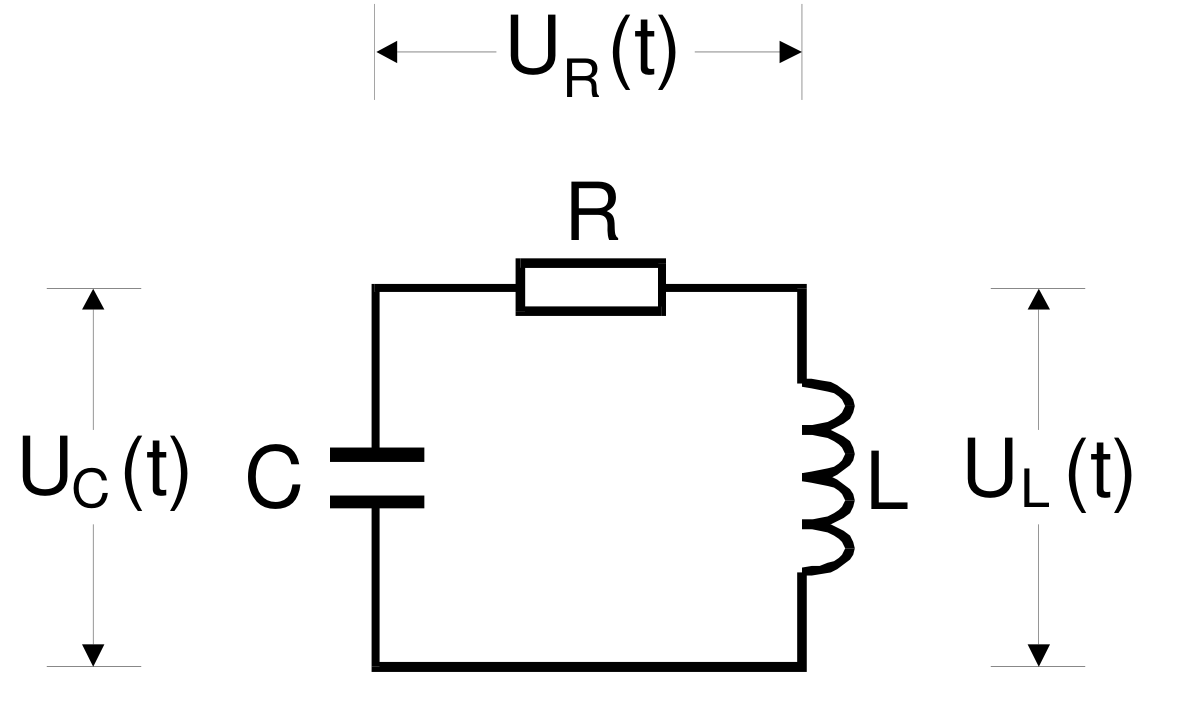
\includegraphics[width=0.5\textwidth]{Abbildungen/ged_Schwingkreis_Schema.png}
    \caption{Ein gedämpfter Schwingkreis \cite{man:v354}.}
    \label{fig:ged_Schwingkreis_Schema}
\end{figure}
Aus den Kirchhoffschen Regeln lässt sich eine Differenzialgleichung zweiter Ordnung für den gedämpften Schwingkreis herleiten.
Sie lautet
\begin{align}
    \frac{\diff^2 I}{\diff t^2}+ \frac{R}{L} \frac{\diff I}{\diff t} + \frac{1}{LC}I = 0 . 
    \label{eq:Hom_DGL}
\end{align}
Mit dem Ansatz
\begin{align*}
    I(t) = U \exp(i\omega t) & U, I \in \mathbb{C} 
\end{align*}
ergibt sich
\begin{align*}
    (- \omega^2 + i \frac{R}{L} \omega + \frac{1}{LC}I) U \exp(i\omega t)  = 0 .
\end{align*}
Für die Konstante $\omega$ ergibt sich also einer der beiden Werte
\begin{align*}
    \omega_{1,2} = i \frac{R}{2L} \pm \sqrt{\frac{1}{LC}-\frac{R^2}{4L^2}}.
\end{align*}
Zwei praktische Abkürzungen werden definiert:
\begin{align*}
    2\pi \mu &:= \frac{R}{2L} & 2 \pi \stackrel{~}{\nu} &:=  \sqrt{\frac{1}{LC}-\frac{R^2}{4L^2}}
\end{align*}
% $I(t)$ lässt sich schreiben als
% \begin{align}
%     I(t)= e^{}
% \end{align}
%%% Vielleicht ein unnötiges Detail 
Für die Lösung der Differenzialgleichung ist es wichtig ob der Therm für $\omega$ eine reelle oder eine komplexe Zahl ist.

Im ersten Fall ist $\stackrel{~}{\nu}$ reel d.h.
\begin{align*}
    \frac{1}{LC} > \frac{R^2}{4L^2}
\end{align*}
Die Lösung für diesen fall lautet
\begin{align}
    I(t) = A_0 e^{-2\pi \mu t}\cos(2 \pi \nu t + \eta)
    \label{eq:Schwingfall}
\end{align}
und ist eine gedämpfte Schwingung.
%%%%%%%%%%%%%%%%%%%%%% blink
\begin{figure}
    \centering
    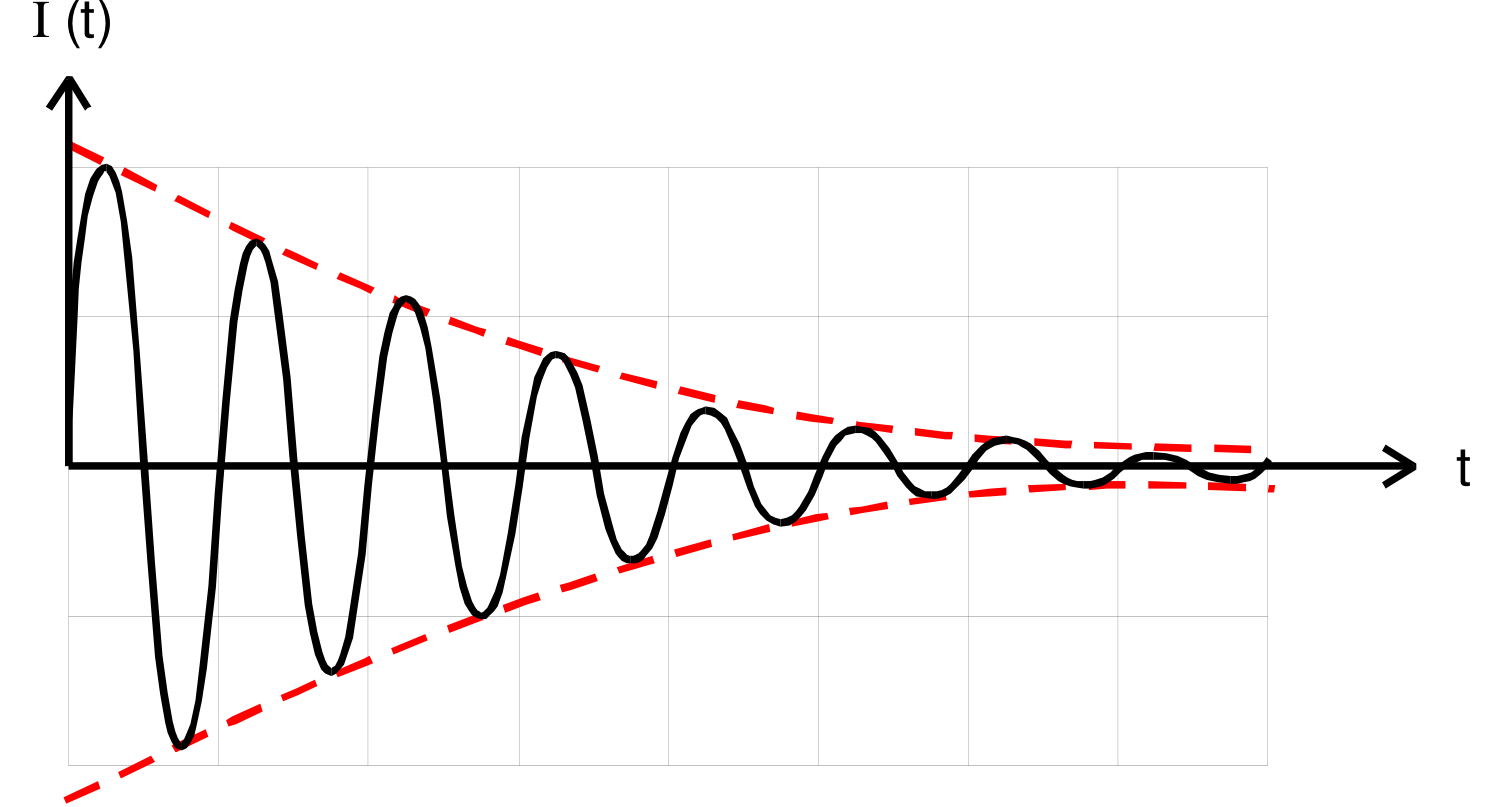
\includegraphics[width=0.7\textwidth]{Abbildungen/Schwingfall_Funktion.png}
    \caption{Die Funktion im Schwingfall bei niedriger Dämpfung \cite{man:v354}.}
    \label{fig:Schwingfall}
\end{figure}
In Abbildung \ref{fig:Schwingfall} wird die Form dieser Schwingung mit der einhüllenden e-Funktion und dem schwingenden Anteil dargestellt.
Die Amplitude der Schwingung geht mit der Zeit exponentiell gegen 0. Die Schwingungsdauer hat den Wert
\begin{subequations}\label{eq:Schwingungsdauer}
\begin{align}
    T = \frac{1}{\nu} = \frac{2\pi}{\sqrt{1/LC - R^2 / 4L^2}}. \tag{\ref{eq:Schwingungsdauer}} 
\end{align}
Sie kann mit der Schwingdauer des ungedämpften Harmonischen Oszillator angenähert werden.
    \begin{align}  
        T \simeq T_0 = \frac{2\pi}{\omega_0} = 2\pi \sqrt{LC} \label{eq:Schwingungsdauer_0}
    \end{align}
\end{subequations} 
Die Abnahmegeschwindigkeit wird durch den Parameter $\mu$ charakterisiert.
Die Abklingdauer $T_\text{ex}$ ist die Zeit zu der die Amplitude $A$ den Wert $1/e A_0$ erreicht.
Aus der Formel lassen sich Rückschlüsse auf den wirkenden Widerstand ziehen.
\begin{align}
    T_\text{ex} := \frac{1}{2\pi mu}= \frac{2L}{R}
    \label{eq:Abklingdauer}
\end{align} 
%
Im anderen Fall ist $\stackrel{~}{\nu}$ rein imaginär bzw.
\begin{align*}
    \frac{1}{LC} < \frac{R^2}{4L^2}
\end{align*}

Die entstehende Lösung heißt aperiodische Dämpfung und kann je nach Anfangsbedingungen einen Extremwert erreichen bevor sie
proportional zu
\begin{align*}
    exp \left(-  \left( R/2L - \sqrt{R^2 / 4 L^2 - 1/LC} \right) t \right)
\end{align*}
verläuft und einem einfachen Relaxationsverhalten folgt (vgl. Abb. \ref{fig:Abfall_Funktionen} durchgezogene Linien).
%%%%%%%%%%%%%%%%%%%%%% blink
\begin{figure}
    \centering
    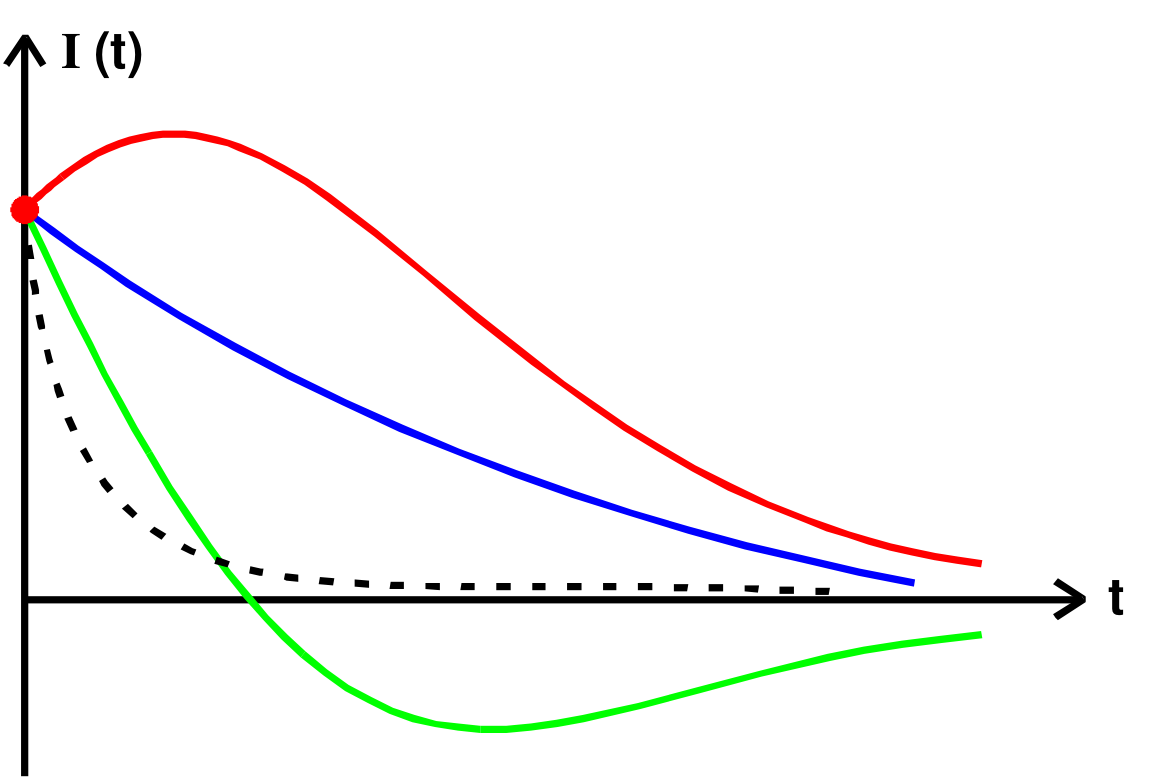
\includegraphics[width=0.7\textwidth]{Abbildungen/Abfall_Funktionen.png}
    \caption{Einige aperiodische Funktionen bei großer Dämpfung und im aperiodischen Grenzfall \cite{man:v354}.}
    \label{fig:Abfall_Funktionen}
\end{figure}
Wenn $\stackrel{~}{\nu} = 0$ ist also
\begin{align}
    \frac{1}{LC} = \frac{R^2}{4L^2}
    \label{eq:ap_bed}
\end{align}
gilt ist der aperiodische Grenzfall erreicht.
Hier geht $I(t)$ ohne Überschwingung am schnellsten gegen Null (Abb. \ref{fig:Abfall_Funktionen} gestrichelte Linie).
Die Lösung hierzu ist
\begin{align}
    I(t) = A e^{- \frac{R}{2L} t} = A e^{- \frac{t}{\sqrt{LC}}} .
    \label{eq:Aperiodischer_Grenzfall}
\end{align}